\begin{refsection}

\chapter{Scaling sequence library multiplexing with semi-automated liquid handling}

\chapterauthor{Russell Y. Neches, Mary Huang}

\section{Author contributions}

This project was conceived of, initiated and carried out by Russell Y. Neches in response to a problem initially posed by Aaron E. Darling in 2010. The process was refined over several years with input and from Martijn Elserman, Erik de Bruijn and Siert Wijnia from Ultimaker BV, who also donated components, and Mary Huang who advised on strategies for achieving water-tight 3D prints. The software was written by Russell Y. Neches and Mary Huang. Timing data for human liquid handling operations was collected by Ashanti M. Robinson. The manuscript was written by Russell Y. Neches and edited by Mary Huang.

\section{Abstract}

When scaling molecular protocols to very large sample sizes ($N > 10,000$), any step that requires each sample to be treated uniquely becomes a major obstacle. Here, we examine the construction of genomic sequencing libraries, and observe that only one step -- normalizing DNA concentrations -- requires unique handling. Rather than executing a unique liquid handling operation on each sample, we instead fabricate single-use microtiter plates with volumes calibrated for each sample. Liquid handling operations are then identical across all samples, allowing the use of multichannel pipettes. Because many custom plates can be 3D printed simultaneously, savings are realized in cost and time.

\section{Introduction}

Robotic liquid handling is capable of scaling the number and complexity of many tasks in molecular biology beyond what is practical for a human operator to undertake. However, the technology has seen limited applications in research settings due to the complexity of developing and debugging protocols. In particular, small academic laboratories often exploit their greater flexibility with respect to larger operations by making frequent adaptations and optimizations to molecular protocols. Small labs often rely on a very diverse repertoire of protocols relative to their size. It is often not worth the time and trouble to develop automated protocols. Along with the high cost of robotic liquid handling systems, the impracticality of using them means that molecular work in most research settings is an entirely manual operation. The scientific consequences are significant; projects that can be undertaken in academic laboratories are often limited in scale to what can be achieved by main force. A middle way between fully robotic automation and entirely manual bench work could open up new areas of research.

We observe that the great majority of steps in many important molecular protocols are identical among all samples. Often, only one or two steps require that individual samples be handled in a unique way. By automating only these steps, it is possible to adapt the protocol to simple parallelization using multi-channel pipetters and to eliminate tedious and error-prone manual lookup operations. Here, we present a simple example of a semi-automated protocol for sequencing library construction for genomic DNA using single use 3D printed parts to automate the normalization of eluent concentrations.

\section{Materials \& Methods}

DNA is extracted in 96-well plates and concentrations are read using a colormetric assay on microplate reader. Concentrations are saved in CSV format, and uploaded to a web application with user-selected ranges for the target concentration and pipetting volume. The application runs locally in the client's browser in {\tt JavaScript}, so the server only serves static documents. The application calculates volume of water required to dilute each pipetted volume of each sample to the the target concentration, and select a 3D modeling component with the corresponding volume. The 3D modeling components are assembled into a fully realized 3D model of a custom 96-well plate and displayed in the browser using {\tt three.js}, \cite{cabello2010three} and the user may then download the model as an STL file for 3D printing (\ref{DP_fig1}). 

\begin{figure}
    \centering
    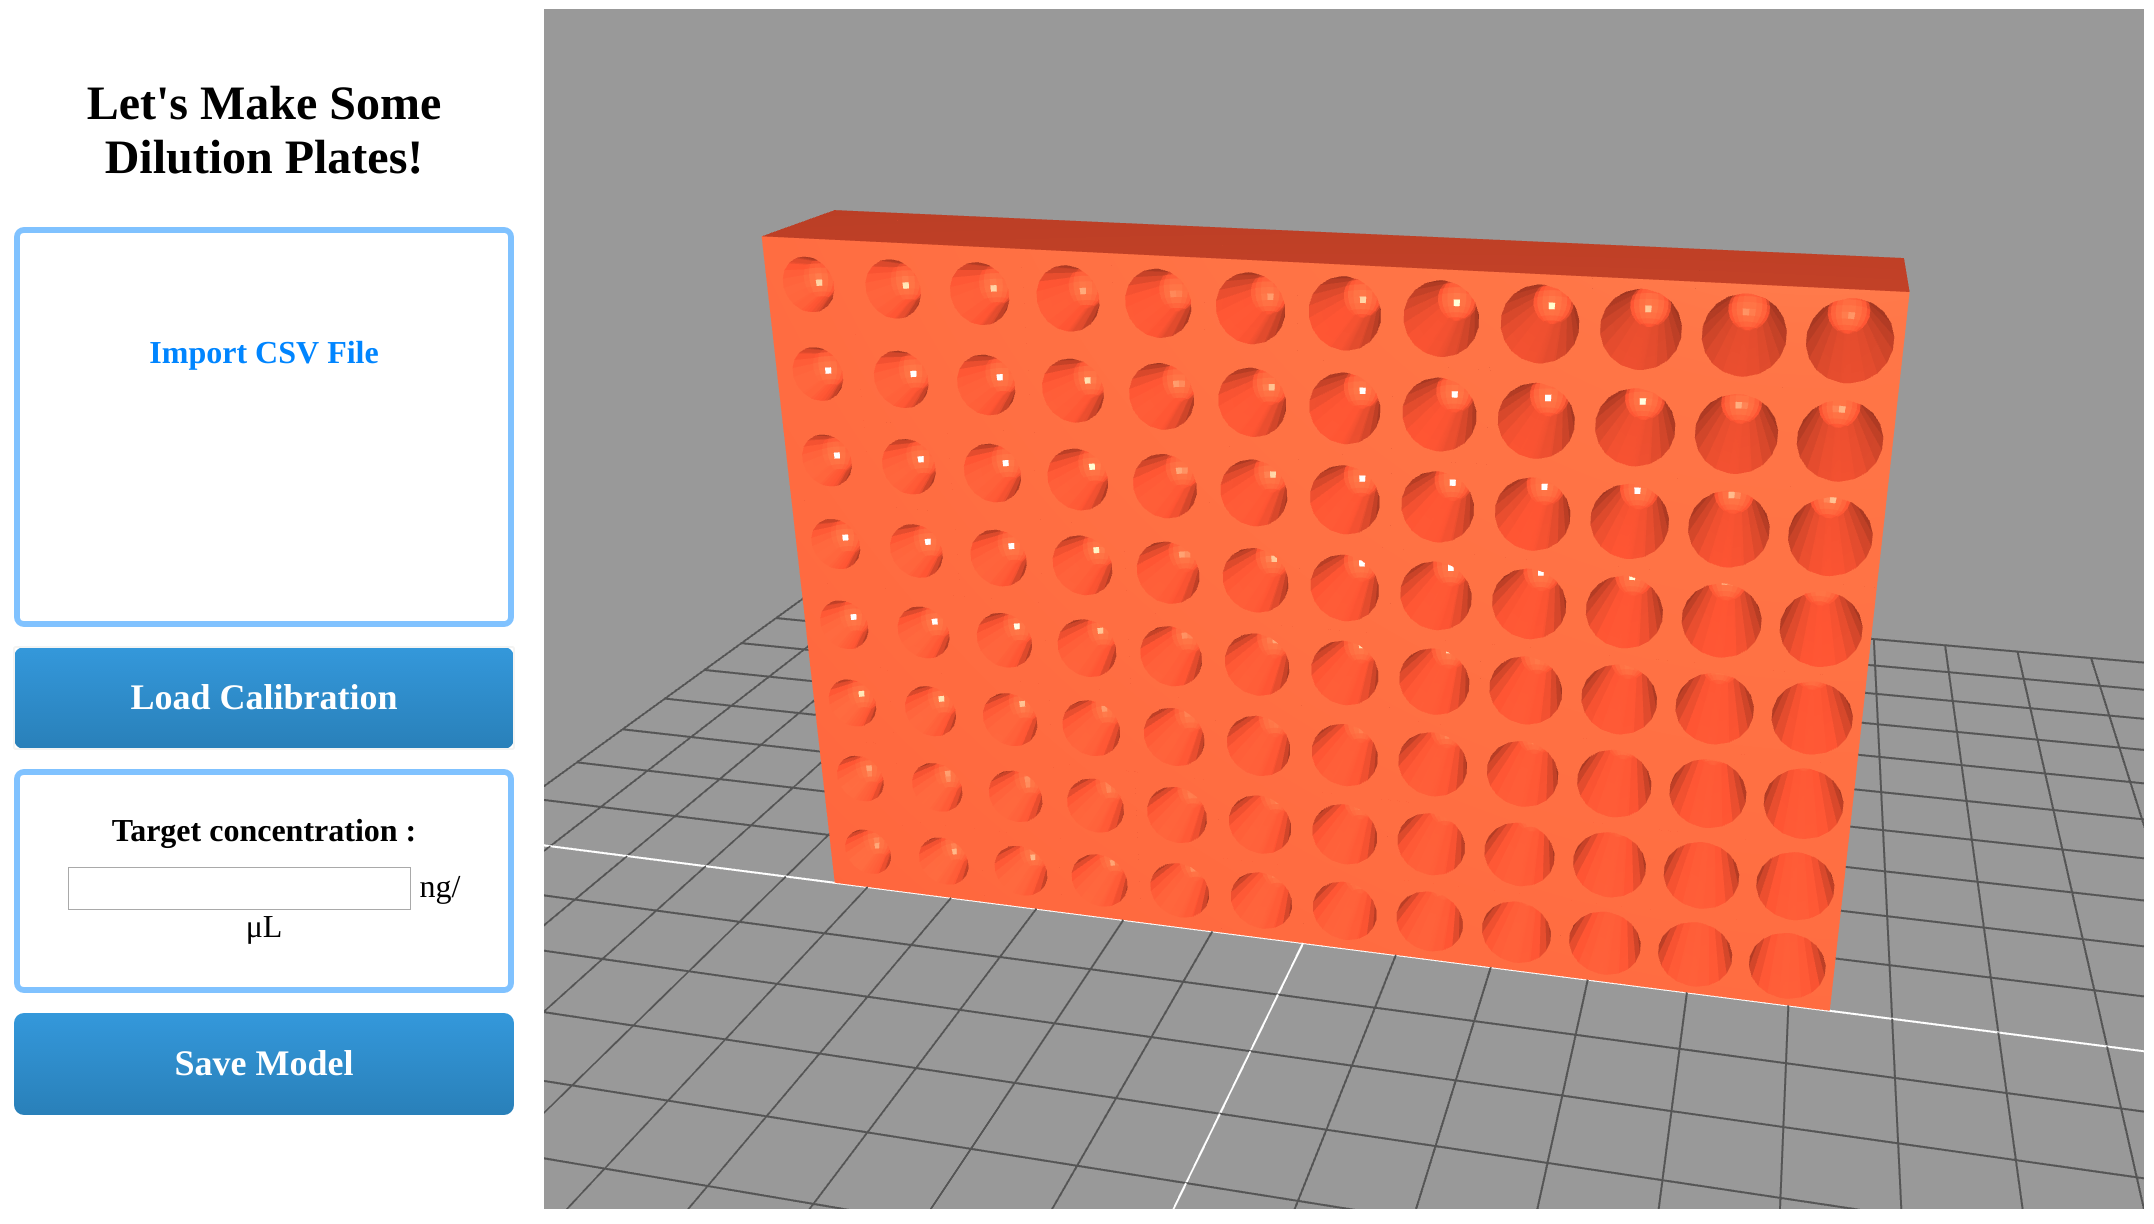
\includegraphics[width=\textwidth]{DilutionPlates/figures/fig1}
    \caption{\textbf{Prototype {\tt DilutionPlates} web applicaiton.}}
    \label{DP_fig1}
\end{figure}

It has been previously reported that the fused deposition modeling 3D printing process (FDM) using thermoplastics like polylactic acid (PLA) and acrylonitrile butadiene styrene (ABS) results in sterile components. \cite{neches2016intrinsic} With a sterile handling technique, the 3D printed plates can be used directly without any additional processing, cleaning or treatment.

The 3D printed plate is transfered from the 3D printer to the work area and filled with laboratory grade water. This can be accomplished quickly by placing the 3D printed part in a tray, and simply pouring water over the top and allowing the excess to overflow. The wells are then leveled by tapping the plate and shaking off the excess. A multichannel pipetter is then used to remove liquid to create a working headspace in each well (100\si{\micro\liter} by default, configurable by the user). The pipetter is then set to the working volume for the dilution reported by the web application, and uniform volumes of sample DNA are transfered from the extraction plate to the 3D printed dilution plate, pipetting up and down to mix thoroughly. The dilution plate now contains DNA at uniform concentrations but different volumes. If desired, the pipetter may then be reset to the maximum working volume reported by the application, and the normalized samples can be transfered to a standard 96-well plate for storage or downstream processing.

\subfile{DilutionPlates/table2}

Using this procedure, a human operator can process a single plate in about five minutes using with a 12-channel pipetter, compared to an hour or more using a traditional approach with single-channel pipetter. By processing large batch of dilution plates together, the time per plate could be reduced to as little as a minute or two. Processing several plates using traditional approach would realize almost no reduction in time per plate, and would represent a very tedious and unpleasant task. These gains are realized by eliminating almost all of the steps where the operator must look up a volume from a table and set the pipetter accordingly and by enabling the use of a multichannel pipetter.

\section{Discussion}

In 2014, our lab produced a sequencing run that yielded 41.7 billion base pairs at the cost of \$2,346. The project in question targeted an organism with a large ($>800$ megabase) genome, and so it achieved a coverage of about $50\times$. Most bacteria and archaea have genomes between one and ten megabases. In principle, it should be possible to multiplex hundreds, or perhaps thousands, of isolate genomes into a single high-throughput sequencing run. For smaller entities, such as amplicons, viruses, plasmids or synthetic constructs, modern sequencing platforms have the capacity to process hundreds of thousands or millions of multiplexed samples. The reality, unfortunately, is that there are impediments to scaling a multiplexed run to this extent, resulting in wasted sequencing capacity and missed scientific opportunities.

The first bottleneck is DNA extraction. The DNA extraction kits on which many fields have standardized cost between \$1 and \$10 per sample. Including controls, a project with more than 470 multiplexed samples using PowerSoil kit\footnote{The 96-well format version of the Qiagen DNeasy PowerSoil kit costs \$5 per sample :\\ \url{https://www.qiagen.com/us/shop/sample-technologies/dna/dna-preparation/dneasy-powersoil-htp-96-kit/}} would have to budget more money for DNA extraction than sequencing. For many projects, the DNA extraction bottleneck can be avoided by substituting in-house protocols for kit-based protocols, or by selecting downstream steps that are compatible with raw cell lysate or supernatent.

The second bottleneck is barcoding. At high concentration, oligos for sequencing and barcoding cost between \$9.25 \$100 each.\footnote{Assuming \$0.37 per base pair and 25 base pairs at 250 \si{\nano\mole} DNA at the low end, or \$2 per base pair and 50 base pairs at 1 \si{\micro\mole} DNA at the high end.} Oligo synthesis costs will exceed sequencing costs somewehere between 23 and 93 samples, though oligos can be used for many sequencing runs. If one were to spend an equal amount on PowerSoil DNA extraction kits and sequencing, the oligos for 470 samples would cost at least \$4,347, double the cost of sequencing. Without reagents or labor, sequencing would make up only a quarter of the project cost. The solution to this problem is combinatoric barcoding; barcodes are attached to either end of the sequenced fragments, allowing unique combinations of barcoades to identify samples. With this approach, the number of oligos required scales with the square root of the number of samples required. For 470 samples, 22 oligos would be required, at a cost of at least \$203 (the worst case, \$2,200, is slightly less than the sequencing cost).

The third bottleneck is labor. Obviously, projects with more samples will involve more basic operations. However, to understand how this impedes large-scale multiplexing, it is important to examine in detail what changes about the work as the number of samples increases. As an example, let us consider a project that uses transposon-based tagmentation \cite{adey2010rapid} to sequence a large number of genomes from bacterial isolate cultures. The tagmentation process is robust enough to function on ``dirty'' DNA, and so we use the supernatent of heat-treated lysate instead of a DNA extraction kit. Here is a schematic protocol for preparing genomic libraries :

\begin{itemize}[noitemsep]
\item \textbf{aliquot samples into bead-beating plates}
\item bead beat samples
\item incubate
\item centrifuge lysate
\item aliquot supernatent to clear bottom plates
\item quantify DNA concentration on plate reader
\item calculate dilution ratio to normalize all samples
\item \textbf{pipette buffer into reaction plates}
\item \textbf{pipette sample into reaction plates}
\item aliquot oligos
\item aliquot reagents
\item incubate
\item heat kill reagents
\item combine samples into multiplexed library
\item quantify and normalize library
\item sequence
\end{itemize}

\noindent The steps that require treating each sample individually are in bold. The first such step is sample intake, which is unavoidable, and many laboratories have procedures to optimize sample intake using standardization and parallelization. Citizen science projects may reduce this burden with protocols that shift some sample intake tasks to the larger group (for example, by using pre-indexed plates and a web-based registration process). 

The second two steps, in which the DNA yielded from each sample is diluted to a standard concentration, scale linearly with the number of samples. For every sample, the operator must perform at least thirteen separate operations :

\subfile{DilutionPlates/table1}

\noindent This assumes the operator does not change tips for the pipetter used for buffer, which may be poor practice. It takes about 

\section{Conclusion}


Low-cost 3D printers can now be purchased for under \$200, placing them in the same cost category as a benchtop mini centrifuge. Highly capable ``pro-sumer'' 3D printers cost less than a set of pipetters. The high temperatures and pressures required for 3D printing with the thermoplastic fused deposition modeling process yield sterile components without any subsequent treatment. The potential for reduced costs and improved availability of disposable plastic labware is compelling in its own right, but the true potential of 3D printing that it is just as easy to print a custom component as a standard one. The challenge is in the software. While it is often not practical to design custom components from scratch, users could generate custom variations on a design pattern based on a small number of parameters. Parameterized design of parts for 3D printing lends itself to a kind of flexible, small-scale automation that is presently absent in academic research settings.

\printbibliography[heading=subbibliography]

\end{refsection}